%! Author = amatarazzo
%! Date = 10/03/24


\chapter{Introduction to Large Language Models}
\label{ch:introduction}


\section{Definition and Overview}
\label{sec:definition-and-overview}

In the contemporary landscape of artificial intelligence, Large Language Models (LLMs) stand out as monumental achievements, revolutionizing natural language processing.
These models, characterized by their immense scale and complexity, have become pivotal in understanding and generating human-like text.
At their core, LLMs are designed to comprehend, learn, and generate coherent and contextually relevant language on a scale previously unparalleled.

Historically, the development of Language Models (LMs) has been rooted in the quest to understand and replicate human language and 4 main stages can be identified:
\begin{enumerate}
    \item \textbf{Statistical Language Models:} {These models were developed to capture the statistical properties of language, such as word frequencies and co-occurrences, to predict the likelihood of a given sequence of words based on the Markov assumption, which states that the probability of a word depends only on the previous $n$ words.
    If the context length $n$ is fixed, the model is called an $n$-gram model.\\
    However, these models are limited by the exponential number of transitions probabilities to be estimated, and the Markov assumption itself, which it may not always hold true in the complexity of natural languages.
    Language understanding often involves capturing dependencies over longer distances than what the Markov assumption allows for. Models that consider broader contexts, such as recurrent neural networks (RNNs) and transformers, have been developed to address these long-range dependencies in language processing tasks.}
    \item \textbf{Neural Language Models:} {The advent of neural networks led to the development of language models that utilized neural architectures to capture the complex patterns and dependencies present in language.
    These models, such as recurrent neural networks (RNNs) and long short-term memory (LSTM) networks, were able to capture long-range dependencies and contextual information, enabling them to generate coherent and contextually relevant text.
    The work \cite{nlm} introduced the concept of $distributed representation$ of words and build the word prediction function of the distributed word vectors.
    Later, word2vec~\cite{word2vec, word2vec2} introduced the word2vec model, which is a shallow, two-layer neural network that is trained to reconstruct linguistic contexts of words.
    These models were a significant leap forward in the development of language models, representing a shift from word sequencing to learning representation.}
    \item \textbf{Pre-trained language models (PLM):} {The development of pre-trained language models (PLMs) marked a significant milestone in the evolution of language models.
    These models were trained on large corpora of data, in an unsupervised or self-supervised manner, before being fine-tuned on specific tasks. The idea is to pre-train a model on a diverse set of data and then transfer its knowledge to a narrower task by fine-tuning on a smaller, task-specific dataset.
    ELMo (Embeddings from Language Models)~\cite{elmo} was one of the first PLMs, which used a bidirectional LSTM to generate word embeddings (instead of learning fixed word representations).
    The work \cite{bert} introduced BERT (Bidirectional Encoder Representations from Transformers), which is a transformer-based model that is pre-trained on a large corpus of text and then fine-tuned on specific tasks.
    BERT was a significant advancement in the field of natural language processing, as it demonstrated the potential of pre-trained language models to achieve state-of-the-art performance on a wide range of tasks.
    These studies introduced the $"pre-training and fine-tuning"$ paradigm, which has become a standard practice in the development of language models and inspired great number of models, such as GPT-2~\cite{gpt2}, GPT-3~\cite{gpt3}, T5~\cite{t5}, and many others.
    }
    \item \textbf{Large Language Models (LLM):} {The emergence of large language models, characterized by their immense scale and complexity, has redefined the capabilities of language processing systems.
    Studies find that the performance of language models improves as the number of parameters ($e.g.$ model size) or data size increases, a phenomenon known as the scaling law in large language models.
    Many LLMs are built on the transformer architecture, which is designed to capture long-range dependencies and contextual information in language.
    The transformer architecture has become the foundation for many state-of-the-art language models and, unlike earlier models that were unidirectional (e.g., traditional RNNs), LLMs, especially those based on transformers, are bidirectional. They consider context from both preceding and following words, enhancing their understanding of language.
    LLMs find applications across various domains, including but not limited to:
        \begin{itemize}
            \item \textbf{Text Generation:} Producing coherent and contextually relevant text.
            \item \textbf{Question Answering:} Answering questions based on provided context.
            \item \textbf{Language Translation:} Translating text from one language to another.
            \item \textbf{Summarization:} Creating concise summaries of longer texts.
            \item \textbf{Sentiment Analysis:} Determining the sentiment expressed in a piece of text.
        \end{itemize}
        These large sized PLMs have been shown to outperform their smaller ($e.g.$, 330M-parameters vs 1.5B-parameters) and show surprising capabilities \footnote{Note that a LLM is not necessarily more capable than a small PLM, and emergent abilities may not occur in some LLMs.}, also called emergent abilities~\cite{emergent2}.
        \begin{displayquote}
            Emergence is when quantitative changes in a system result in qualitative changes in behavior~\cite{emergent1}.
        \end{displayquote}
        These emergent abilities include, but are not limited to, the ability to perform tasks for which they were not explicitly trained, such as translation, summarization, and question-answering, and to generalize to new tasks and domains, such as zero-shot learning \footnote{it refers to a machine learning scenario where a model makes predictions or performs tasks for classes or examples it has never seen during training}, few-shot learning \footnote{it involves training a model with a very small number of examples per class, usually much fewer than what traditional machine learning models require}, and even one-shot learning \footnote{it is a specific case of few-shot learning where the model is trained with only one example per class} learning.
        Three tipical examples of emergent abilities are:
        \begin{enumerate}
            \item \textbf{In-context learning:} {this ability has been formally observed in GPT-3, which is provided with a natural language instruction or task demonstrations, it can generate the expected output for test instances by completing the word sequence of the input text. Importantly, this can be achieved without requiring additional training or gradient updates \footnote{Recent study shows that in-context learning implicitly performs meta optimisation through the attention mechaninsm \cite{icl}}.
                \begin{quote}
                    \textbf{Language Translation:} \\
                    \textit{Input:} {\enquote{Translate the following English text to French: `The quick brown fox jumps over the lazy dog.'}} \\
                    \textit{Output:} {\enquote{Le renard brun rapide saute par-dessus le chien paresseux.}}\\
                    \textbf{Arithmetic Tasks:} \\
                    \textit{Input:} {\enquote{What is the sum of 42 and 63?}} \\
                    \textit{Output:} {\enquote{The sum of 42 and 63 is 105.}}
                \end{quote}
            }
            \item \textbf{Instruction following:}{
                Through the process called instruction tuning, LLMs exhibits strong performance on unseen tasks described through natural language instructions \cite{instruction1, ouyang2022training, wei2022fine}.
                This approach involves fine-tuning the model using a diverse set of multitask datasets, each accompanied by detailed natural language descriptions. The result is an LLM that effectively interprets and follows task instructions for new and unseen tasks without relying on explicit examples, thereby showcasing enhanced generalization capabilities.
                Experiments detailed in \cite{wei2022fine} demonstrate that LaMDA-PT, fine-tuned with instructions, begins to outperform its untuned counterpart significantly when the model size reaches 68 billion parameters. However, this performance gain is not observed for model sizes of 8 billion or smaller. Furthermore, recent research \cite{chung2022scaling} highlights that a model size of at least 62 billion parameters is necessary for PaLM to excel across various tasks in evaluation benchmarks like MMLU, BBH, TyDiQA, and MGSM. Nevertheless, it is noted that certain specific tasks, such as MMLU, might suffice with a much smaller model size, emphasizing the nuanced relationship between model size and task performance.
            }
            \item \textbf{Step-by-step reasoning:} { For small LMs, it is usually difficult to solve complex tasks that involve multiple reasoning steps, e.g., mathematical word problems.
            In contrast, the chain-of-thought (CoT) prompting strategy \cite{wei2022chain} empowers Large Language Models (LLMs) to surmount these challenges. By leveraging the CoT prompting mechanism, which involves intermediate reasoning steps to derive the final solution, LLMs exhibit proficiency in tasks that demand intricate cognitive processes. This capability is speculated to be honed through training on code \citation{wei2022chain}. Empirical findings \citation{wei2022chain} demonstrate that the employment of CoT prompting yields performance gains, particularly on arithmetic reasoning benchmarks, when applied to variants of models like PaLM and LaMDA, especially with a model size surpassing 60B. The advantages of CoT prompting become more pronounced as the model size exceeds 100B. Furthermore, the effectiveness of CoT prompting exhibits variability across different tasks, with performance improvement observed in the order of GSM8K~\textgreater~MAWPS~\textgreater~SWAMP for PaLM \citation{wei2022chain}.
            }
        \end{enumerate}
    }
\end{enumerate}
The advent of LLMs has led to a paradigm shift in the field of natural language processing, with applications ranging from machine translation to text summarization, and from question-answering systems to language generation.
The development of LLMs has been driven by the exponential growth of data and computational resources, which has enabled the training of models with billions of parameters.
The scale of these models has enabled them to capture complex patterns in language and generate coherent and contextually relevant text.

The potential of LLMs is vast, and their impact on the field of natural language processing is profound.
The advent of ChatGPT~\cite{chatgpt} and GPT-4~\cite{gpt4} has further expanded the capabilities of LLMs, leads to the rethinking of the possibilities of artificial general intelligence (AGI).
Talking about NLP, LLMs can serve somewhat as a general-purpose language task solver.
In the IR field, LLMs can be used to improve the performance of information retrieval systems, through AI chatbots ($i.e.$, ChatGPT), and New Bing \footnote{https://www.microsoft.com/it-it/bing?form=MA13FV}.
In the CV field, LLMs can be used to improve the performance of computer vision systems, through multimodal models /footnote{
    Models designed to process and understand information from multiple modalities or sources ($e.g$, text, image, audio, video).
    Multimodal models aim to handle and integrate data from two or more of these modalities.
} ($i.e.$, CLIP~\cite{clip} \footnote{Contrastive Language–Image Pre-training} and DALL-E~\cite{dall-e}).

The purpose of this thesis is to provide an overview of the current state of LLMs, including their capabilities, limitations, and potential applications, and it's mainly based on this~\cite{survey} work.
The thesis will also explore and compare the abilities of different LLMs, focusing on the impact of various parameters on their performance.


\section{Scaling Law}
\label{sec:scaling-law-in-large-language-models}

The Scaling Law in Large Language Models (LLMs) constitutes a fundamental principle that underlines their development and performance.
At its essence, the scaling law posits that as the size of language models increases, their capabilities and performance on linguistic tasks exhibit a disproportionately positive growth.
This concept has become a guiding force in pushing the boundaries of language processing and understanding.

As LLMs scale up in terms of parameters, encompassing tens or hundreds of billions, or even trillions, of parameters, they demonstrate an unprecedented ability to generalize from diverse datasets and generate contextually coherent text.
The essence of the scaling law lies in the direct correlation between the size of a language model and the number of parameters it encompasses.
Parameters are the internal variables that the model learns during training, representing the connections and weights that define its understanding of language.
As the number of parameters increases, so does the model's capacity to encapsulate complex linguistic structures.

One of the primary outcomes of adhering to the scaling law is the substantial improvement in performance across a spectrum of language-related tasks.
From language generation to sentiment analysis, and from question-answering to summarization, larger models consistently outperform their smaller counterparts.
The increased capacity for learning intricate language features enables LLMs to excel in understanding and producing more human-like text.

At the time of writing, most of the LLMs are based on the transformer architecture, where multi-headed self-attention layers are stacked in a very deep neural network.
We'll deep dive into the transformer architecture in the following chapters, but for now, we can say that self-attention is a mechanism to allow a model to weigh different parts of the input sequence differently, capturing dependencies between words.
The multi-headed self-attention mechanism allows the model to capture different types of dependencies and relationships between words, enhancing its understanding of language.
The idea is that different attention heads can focus on different aspects or relationships within the data, allowing the model to capture more nuanced patterns.
Multiple layers of these multi-headed self-attention mechanisms are stacked in a very deep neural network.
Each layer in the stack processes the output of the previous layer, learning hierarchical representations of the input data, capturing increasingly complex relationships and abstractions. \\
Two representative scaling laws for Transformer-based LLMs are the following~\cite{scaling1, scaling2}:
\begin{enumerate}
    \item \textbf{KM scaling law:} {named in this way in \cite{survey} and proposed by the OpenAI team in \cite{scaling1}. Given model size $M$, dataset size $D$, amount of training compute $C$, and a compute budget $c$, the KM scaling law states that the performance of a language model scales as per the following three formulas:

        \begin{center}
            \begin{math}
                L(N)=(\frac{N_c}{N})^{\alpha_N}, \alpha_N \approx 0.076, N_c \approx 8.8 \times 10^{13}
            \end{math}
        \end{center}

        \begin{center}
            \begin{math}
                L(D)=(\frac{D_c}{D})^{\alpha_D}, \alpha_D \approx 0.095, D_c \approx 5.4 \times 10^{13}
            \end{math}
        \end{center}

        \begin{center}
            \begin{math}
                L(C)=(\frac{C_c}{C})^{\alpha_C}, \alpha_C \approx 0.050, C_c \approx 3.1 \times 10^8
            \end{math}
        \end{center}

        where $L(N)$, $L(D)$, and $L(C)$ denotes the cross-entropy loss of the model, the dataset, and the amount of training compute, respectively.
        The three laws were formulated by analyzing the model's performance across a range of data sizes (from 22M to 23B tokens), model sizes (from 768M to 1.5B non-embedding parameters), and training compute, with certain assumptions (e.g., ensuring that the analysis of one factor is not constrained by the other two factors).
        The findings demonstrated a robust interdependence among the three factors influencing model performance.
    }
    \item \textbf{Chincilla scaling law:} {An alternative form of the scaling law has been proposed by the Google DeepMind team in \cite{scaling2} experimenting a large range of model size (70M to 16B) and data sizes (5B to 500B tokens).
    The Chincilla scaling law posits that the performance of a language model scales as per the following formula:

        \[L(N,D) = E + \frac{A}{N^\alpha} + \frac{B}{D^\beta},\]

        where

        \[E=1.69, A=406.4,B = 410.7, \alpha = 0.34, \beta = 0.28\]

        They showed that optimal allocation of compute budget to model size and data size can be derived as follows \footnote{under the constraint \(C \approx 6ND\)}:

        \begin{center}
            \begin{equation}
                N_{opt}(C) = G(\frac{C}{6})^a, D_{opt}(C) = G^{-1}(\frac{C}{6})^b, \label{eq:optimal-allocations}
            \end{equation}
        \end{center}

        where \(a=\frac{\alpha}{\alpha+\beta}, b=\frac{\beta}{\alpha+\beta}\) and G is a scaling coefficient.
        The KM scaling law favors a larger budget allocation in model size than the data size, while the Chinchilla scaling law argues that the two sizes should be increased in equal scales \cite{scaling2}, i.e., having similar values for a and b in \eqref{eq:optimal-allocations}.
    }
\end{enumerate}

Scaling not only boosts performance but also addresses inherent limitations in smaller language models.
Larger models excel in managing long-range dependencies, comprehending ambiguous language constructs, and displaying a nuanced understanding of context---capabilities that smaller models frequently find challenging.

Despite propelling the field of LLMs to new heights, the scaling law comes with computational challenges.
Training extremely large models requires significant computational resources, encompassing both processing power and memory.
This presents practical obstacles, demanding innovations in hardware and distributed training techniques to fully exploit the potential of scaled-up language models.


\section{Prominent Model Families}
\label{sec:promiment-model-families}

The development of Large Language Models (LLMs) has been driven by the emergence of prominent model families, each characterized by its unique architecture and capabilities.
These model families have played a pivotal role in shaping the landscape of language processing and understanding, and have been instrumental in pushing the boundaries of LLMs.

Some of the most prominent large language models (having a size larger than 10B) are depicted in Figure~\ref{fig:llm-evolution}.

\begin{figure}[h!]
    \centering
    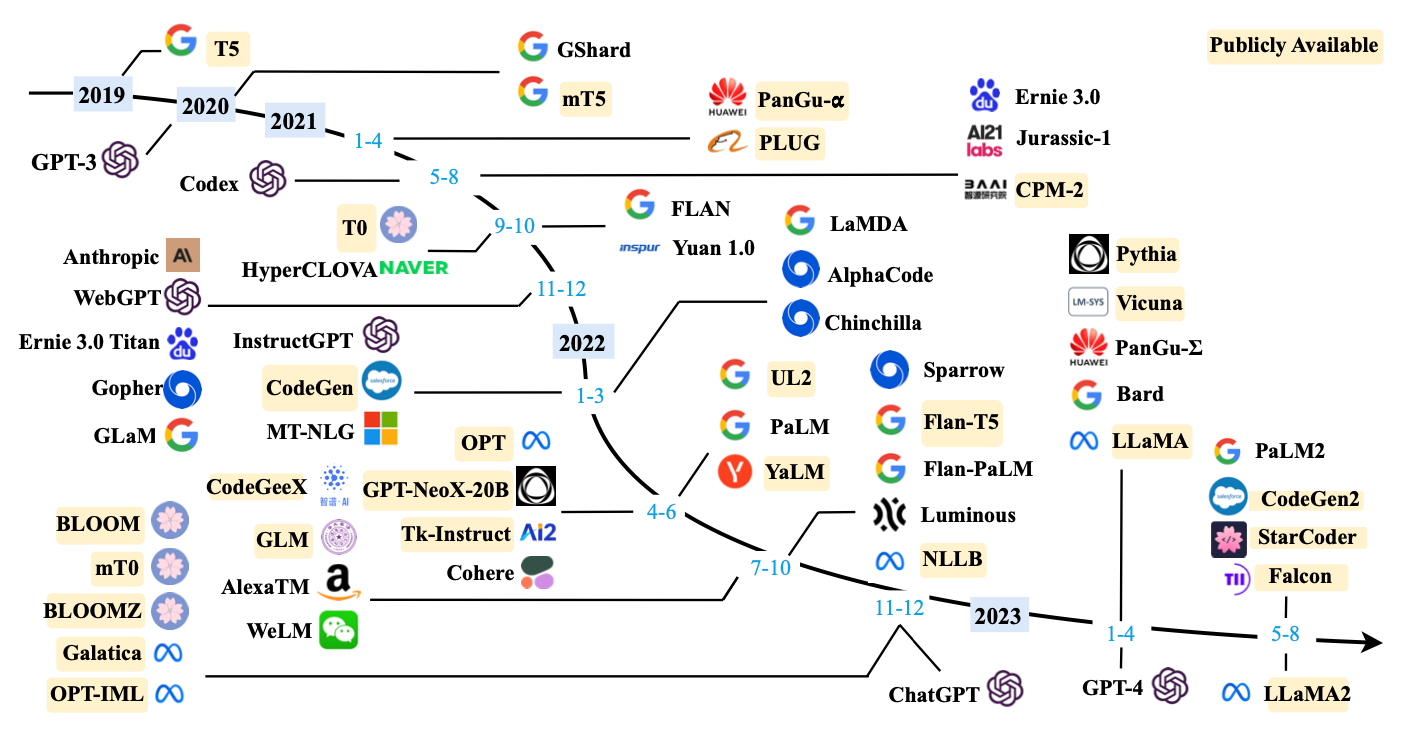
\includegraphics[width=1\textwidth]{public_llm}
    \caption{A diagram showing the evolution of publicly available LLMs.Source: \protect\cite{survey}.}
    \label{fig:llm-evolution}
\end{figure}

\subsection{BERT}
\label{subsec:bert}

Introduced by Google in 2018, BERT~\cite{bert} marked a significant evolution in LLMs by focusing on bidirectional context in text processing.
BERT’s model architecture is a multi-layer bidirectional Transformer encoder based on the original transformer architecture introduced by Vaswani et al.~\cite{vaswani2023attention}.
Unlike its predecessors, BERT analyzes text in both directions (left-to-right and right-to-left), providing a more nuanced understanding of language context.
This bi-directionality enables BERT to achieve state-of-the-art results in a variety of NLP tasks, such as question answering, named entity recognition, and sentiment analysis.
BERT's architecture and training methodology have influenced numerous subsequent models and research initiatives~\cite{bert}.

\begin{figure}[h!]
    \centering
    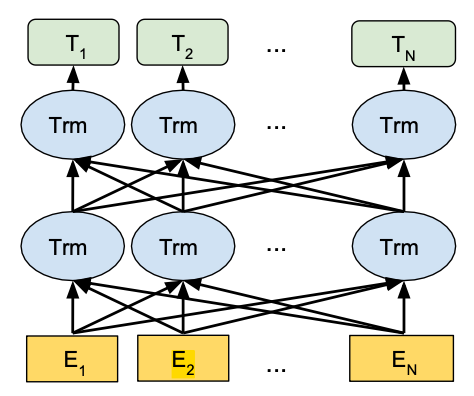
\includegraphics[width=0.5\textwidth]{bert}
    \caption{BERT Architecture: The bottom layer contains the embedding representations \(E_1, E_2, \ldots E_N\), which encode input tokens and serve as the input to the transformer layers (Trm).
    Each transformer bidirectionally processes the input embeddings, and the final output is used for downstream tasks. Source: \protect\cite{bert}.}
    \label{fig:bert-arch}
\end{figure}

Even BERT is built on the transformer architecture~\cite{vaswani2023attention}, which relies heavily on attention mechanisms to understand the context of words in a sentence.
The innovation in BERT is its bidirectional nature and the use of a mechanism called Masked Language Model (MLM). In MLM, some percentage of the input tokens are randomly masked, and the objective is to predict these masked tokens based on their context, leveraging information from both sides of the sequence.
BERT also incorporates a next sentence prediction (NSP) task that helps the model learn relationships between sentences, further enhancing its understanding of context.

BERT's bidirectional context understanding significantly improves its performance on a wide range of NLP tasks, including sentiment analysis, question answering, and named entity recognition.
By pre-training on a large corpus of text and then fine-tuning on specific tasks, BERT can adapt to various domains with relatively little task-specific data, demonstrating impressive transfer learning capabilities.
Its architecture has set a new standard in the field, inspiring a plethora of subsequent models that build on or modify its foundational structure.

Despite its strengths, BERT is not without limitations.
The model's size and complexity require substantial computational resources for training, which can be a barrier for some organizations or researchers.
BERT's focus on context from surrounding text does not inherently solve all challenges in language understanding, particularly with respect to ambiguity, nuance, or the subtleties of human language.
The model can sometimes struggle with tasks requiring extensive world knowledge or reasoning beyond the scope of its training data.

While BERT itself does not exhibit emergent abilities in the same way that scaling up GPT models does, its architecture has enabled new approaches in handling context and language understanding that were not feasible with prior models.
Subsequent iterations and variations of BERT, like RoBERTa (Robustly Optimized BERT Pre-training Approach) and ALBERT (A Lite BERT), have sought to optimize and expand upon BERT's foundational principles, exploring how changes in model size, training methodology, and architecture can influence performance and capabilities.

\subsection{T5}
\label{subsec:t5}

Developed by Google in 2019, T5~\footnote{Text-to-Text Transfer Transformer} re-framed all NLP tasks as a unified text-to-text problem, where every task is cast as generating text from input text.
This approach simplifies the use of a single model across diverse tasks, encouraging a more generalized understanding of language.

\begin{figure}[h!]
    \centering
    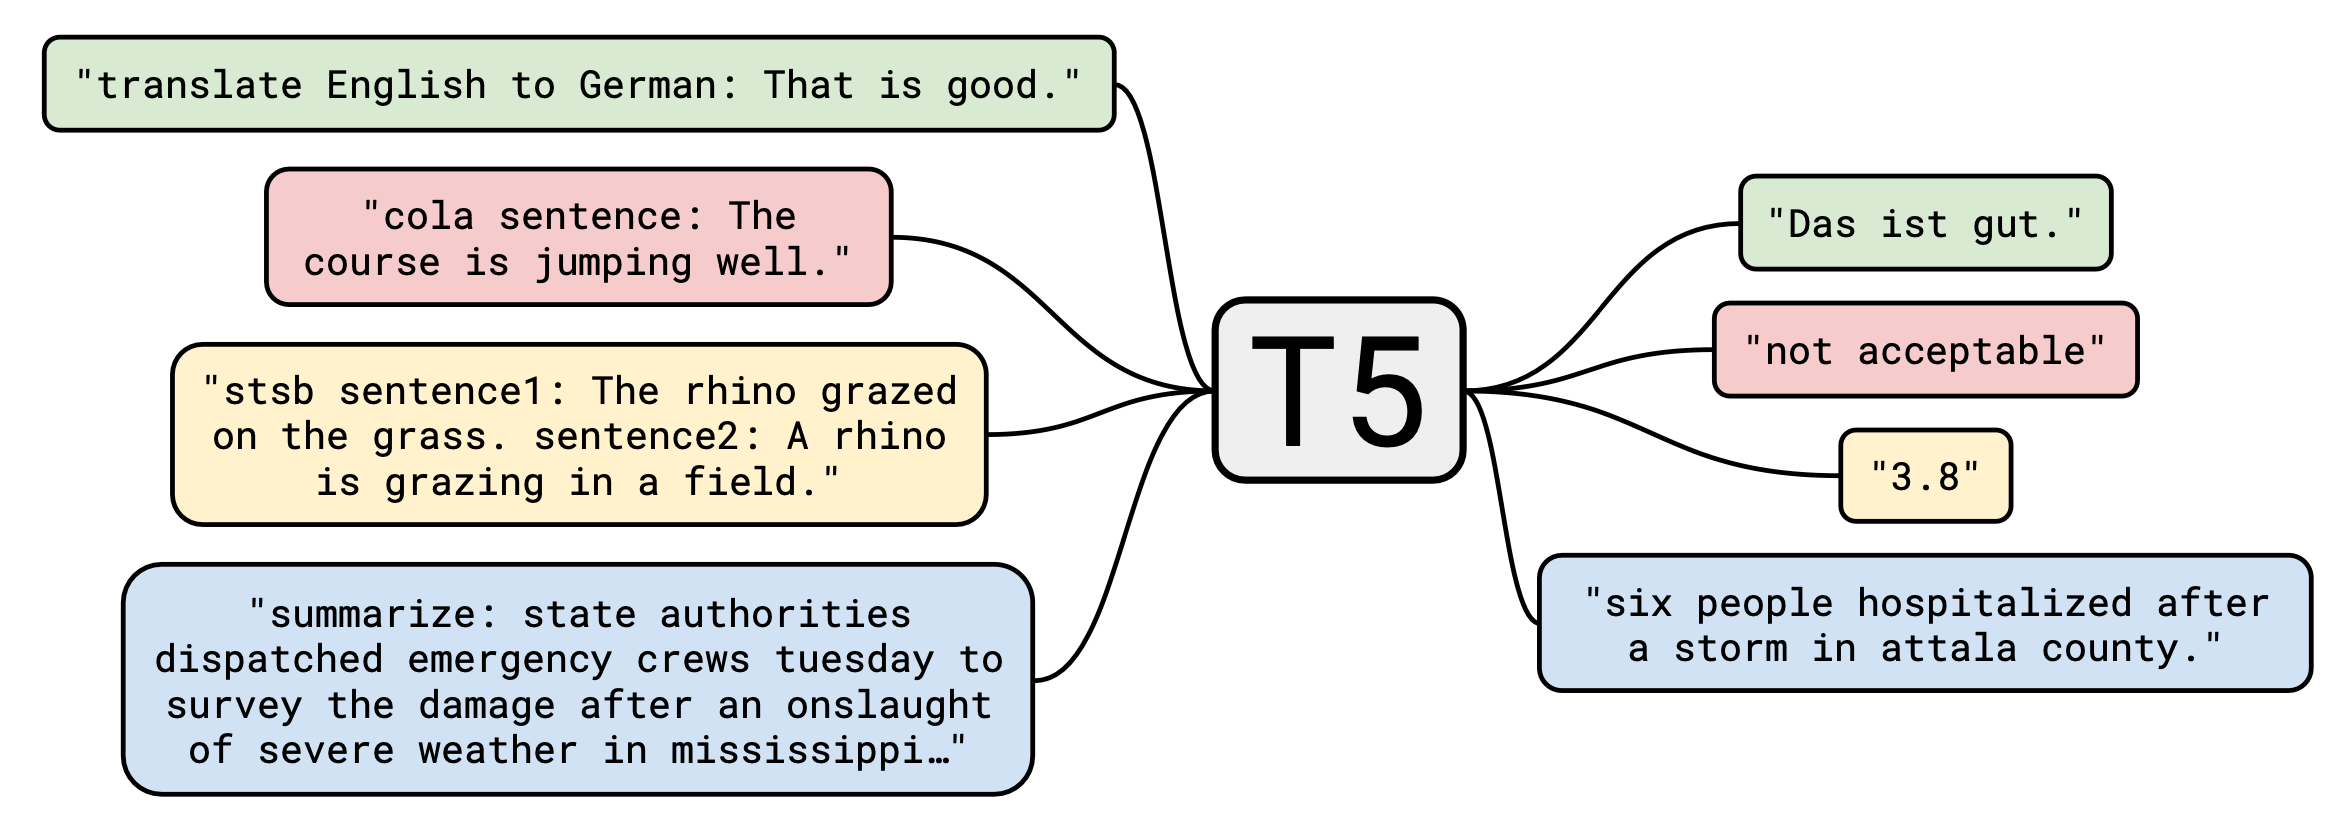
\includegraphics[width=\textwidth]{t5}
    \caption{A diagram of the T5 text-to-text framework. Every task -- including translation, question answering, and classification -- is cast as feeding the model text as input and training it to generate some target text. This allows to use the same model, loss function, hyperparameters, etc. across diverse set of tasks. Source: \protect\cite{t5}.}
    \label{fig:t5-t2t}
\end{figure}

T5 demonstrated its prowess across a range of benchmarks, setting new standards in the field of NLP~\cite{t5}.
It's built on the transformer model, similar to its predecessors like BERT and GPT, leveraging the effective self-attention mechanism for processing sequences of data.
The model is designed to handle a variety of tasks without needing task-specific architectural modifications.
It uses a unified text-to-text framework, where tasks are converted into a format where the input and output are always text strings.
T5 is pre-trained on a multitask mixture of unsupervised and supervised tasks, utilizing a large-scale dataset known as "C4"~\footnote{Colossal Clean Crawled Corpus}.

T5's approach simplifies the process of integrating new tasks into the model's training regime, as they only need to be reformulated into the text-to-text format.
While T5's unified approach offers considerable advantages, it might not be optimally efficient for all types of tasks.
Some tasks could potentially benefit from more specialized model architectures or formats.
The training process for T5 is resource-intensive, requiring substantial computational power, which could be a limiting factor for smaller organizations or independent researchers.
As with other large language models, T5's outputs can sometimes include biases present in the training data, necessitating careful monitoring and potential post-hoc adjustments.

\subsection{GPT Series}
\label{subsec:gpt-series}

Developed by OpenAI, the GPT series has been at the forefront of LLM research.
The original GPT model, introduced in 2018, laid the groundwork with its transformer-based architecture, which significantly improved upon previous models in understanding context and generating text.
It was developed based on a generative, decoder-only Transformer architecture, and adopted a hybrid approach of unsupervised pre-training and supervised fine-tuning.
GPT-2~\cite{gpt2}, released in 2019, expanded on this with 1.5 billion parameters and was trained with a large webpage dataset WebText, demonstrating unprecedented text generation capabilities.
The subsequent GPT-3 model, unveiled in 2020, further pushed the boundaries with 175 billion parameters, showcasing remarkable abilities in generating human-like text, performing language translation, question-answering, and more without task-specific training.
In the research paper on GPT-3~\cite{gpt3}, the authors presented a detailed explanation of the concept known as in-context learning (ICL). This approach enables Large Language Models (LLMs) to function in few-shot or zero-shot scenarios.
ICL empowers LLMs to comprehend tasks when they are described using natural language.
This method aligns the pre-training and application phases of LLMs under a unified framework: during pre-training, the model predicts subsequent text sequences based on prior context.
In contrast, during in-context learning, the model generates the appropriate solution to a task—also in the form of a text sequence—using the provided task instructions and examples.

The GPT series is based on the transformer architecture~\cite{vaswani2023attention}.
This architecture leverages self-attention mechanisms to process input data, which allows the model to weigh the importance of different words within the input context, enhancing its ability to understand and generate language.
GPT models are characterized by their stacked transformer blocks, which consist of multi-headed self-attention layers followed by fully connected feed-forward neural networks.
The series has seen an exponential increase in the number of parameters: GPT with 110 million, GPT-2 with 1.5 billion, and GPT-3 with 175 billion parameters.

GPT models exhibit a remarkable ability to generate coherent and contextually relevant text, simulating human-like writing styles.
They demonstrate strong performance in a wide array of NLP tasks without task-specific data training, showcasing their versatility in few-shot, one-shot, or zero-shot learning scenarios.
The scalability of the architecture has shown that larger models tend to exhibit better performance, capturing subtler patterns in data.

One significant criticism is their data-hungry nature, requiring vast amounts of text data for training, which raises concerns about environmental impact and computational costs.
The models can sometimes generate plausible but factually incorrect or nonsensical information, a phenomenon often referred to as \enquote{hallucination}.
The black-box nature of these models poses challenges in interpretability and transparency, making it difficult to understand how decisions are made or how to correct biases.

GPT-3 demonstrated surprising emergent behaviors, such as improved reasoning, problem-solving, and creative writing, which were not explicitly programmed or observed in its predecessors.
These abilities suggest that scaling up model size can lead to qualitative changes in how models understand and interact with language, although the relationship is not yet fully understood.
OpenAI has explored two major approaches to further improving the GPT-3 model, i.e., training on code data and alignment with human preference, which are detailed as follows:
\begin{enumerate}
    \item \textbf{Training on code data:} {
        This approach involves fine-tuning the model on a diverse set of programming tasks, such as code completion, code generation, and code summarization.
        The model is trained on a large corpus of code data, which includes code snippets, programming languages, and software development documentation.
        The goal is to improve the model's understanding of programming languages and its ability to generate code, thereby enhancing its performance on programming-related tasks.
    }
    \item \textbf{Alignment with human preference:} {
        This approach involves training the model to generate outputs that align with human preferences and values and can be dated back to a work that applied reinforcement learning (RL) \cite{christiano2017deep} (similar to the reward training step in the aligning algorithm of InstructGPT.
    }
\end{enumerate}

\subsubsection{GTP-4}
\label{subsubsec:gpt-4}

GPT-4~\cite{gpt4}, the successor to GPT-3, marks a further advancement in the GPT series developed by OpenAI. While specific details about GPT-4's architecture and capabilities are proprietary, it is known to build upon the foundational concepts of its predecessors, emphasizing scale, capability, and efficiency.
GPT-4 is a multimodal model which can accept image and text inputs and produce text outputs.
Such models are an important area of study as they have the potential to be used in a wide range of applications, such as dialogue systems, text summarization, and machine translation.

\begin{table}[h!]
    \centering
    \caption{Example prompt demonstrating GPT-4's visual input capability. The prompt consists of a question about an image with multiple panels which GPT-4 is able to answer}
    \label{tab:gpt4_example}
    \begin{tabular}{@{}m{2cm}@{}m{10cm}@{}}
        User & What is funny about this image? Describe it panel by panel. \\
        & 
\includegraphics[width=10cm]{gpt4}                          \\
        &                                                             \\
        GPT-4 &
        \begin{tabular}[t]{@{}m{10cm}@{}}
            The image shows a package for a "Lightning Cable" adapter with three panels.                                                                      \\
            Panel 1: A smartphone with a VGA connector (a large, blue, 15-pin connector typically used for computer monitors) plugged into its charging port. \\
            Panel 2: The package for the "Lightning Cable" adapter with a picture of a VGA connector on it.                                                   \\
            Panel 3: A close-up of the VGA connector with a small Lightning connector (used for charging iPhones and other Apple devices) at the end.         \\
            The humor in this image comes from the absurdity of plugging a large, outdated VGA connector into a small, modern smartphone charging port.
        \end{tabular} \\
    \end{tabular}
\end{table}

On the MMLU benchmark~\cite{hendrycks2021measuring}, an English-language suite of multiple-choice questions covering 57 subjects, GPT-4 not only outperforms existing models by a considerable margin in English, but also demonstrates strong performance in other languages.
GPT-4 development was enabled by deep learning infrastructure and optimization methods that behave predictably across a wide range of scales.
This allowed to make predictions about the expected performance of GPT-4 (based on small runs trained in similar ways) that were tested against the final run to increase confidence in our training.
The primary reason is that for very large training runs, it is not feasible to do extensive model-specific tuning.

The prediction GPT-4’s final loss was predicted by fitting a scaling law with an irreducible loss term (as in~\cite{henighan2020scaling}): \(L(C) = aC^b + c\), from models trained using the same methodology but using at most 10,000x less compute than GPT-4.
The fitted scaling law predicted GPT-4’s final loss with high accuracy.
In addition to predicting the final loss, a metric of capability was also predicted.
One such metric is the pass rate on HumanEval dataset~\cite{chen2021evaluating} which measures the ability to write Python function of various complexity.
The approximate power law relationship is \(E_P [\log{pass\_rate(C)}] = \alpha \times C^{-k}\), where k and \(\alpha\) are positive constants, and P is a subset of problems in the dataset.

GPT-4 accepts prompts consisting of both images and text, which -- parallel to the text-only setting -- lets the user specify any vision or language task.
Specifically, the model generates text outputs given inputs consisting of arbitrarily interlaced text and images.

Despite its capabilities, GPT-4 has similar limitations to earlier GPT models: it is not fully reliable (e.g.\ can suffer from \enquote{hallucinations}), has a limited context window, and does not learn from experience.

Care should be taken when using the outputs of GPT-4, particularly in contexts where reliability is important.

\subsection{LLaMA}
\label{subsec:llama}

LLaMA~\footnote{Large Language Model Meta AI} is a language model developed by Meta AI, designed to be a versatile and efficient foundation for a wide range of natural language processing (NLP) tasks.
LLaMA is built on a transformer architecture~\cite{vaswani2023attention}, similar to other large language models, with a range from 7B to 65B parameters.
Main differences between LLaMA and original Tranformer architecture~\cite{vaswani2023attention} are the following:
\begin{enumerate}
    \item \textbf{Pre-normalization\footnote{Inspired by GTP-3 model}} {LLaMA uses pre-normalization, which means that the normalization layer is placed before the self-attention and feed-forward layers.
    Pre-normalization has been shown to improve training stability and convergence in large language models, making it a popular choice for many state-of-the-art models.
    }
    \item \textbf{SwiGLU activation function\footnote{Inspired by PaLM model}} {LLaMA uses the SwiGLU activation function~\cite{shazeer2020glu}, which is a variant of the Gated Linear Unit (GLU) activation function.
    SwiGLU has been shown to improve the performance of large language models by enhancing the flow of information through the network.
    }
    \item \textbf{Rotary Embeddinsgs\footnote{Inspired by GPTNeo model}} {LLaMA uses rotary embeddings~\cite{su2021roformer}, which are a type of positional encoding that helps the model capture long-range dependencies in the input data.
    }
\end{enumerate}

\begin{table}[ht]
    \centering
    \caption{Model sizes, architectures, and optimization hyper-parameters. Source: \protect\cite{touvron2023llama}. }
    \label{tab:llama-model-params}
    \begin{tabular}{@{}ccccccc@{}}
        \toprule
        params & dimension & n heads & n layers & learning rate          & batch size & n tokens \\
        \midrule
        6.7B     & 4096      & 32      & 32       & \(3.0 \times 10^{-4}\) & 4M         & 1.0T     \\
        13.0B    & 5120      & 40      & 40       & \(3.0 \times 10^{-4}\) & 4M         & 1.0T     \\
        32.5B    & 6656      & 52      & 60       & \(1.5 \times 10^{-4}\) & 4M         & 1.4T     \\
        65.2B    & 8192      & 64      & 80       & \(1.5 \times 10^{-4}\) & 4M         & 1.4T     \\
        \bottomrule
    \end{tabular}
\end{table}

Based on the LLaMA paper~\cite{touvron2023llama}, even though LLaMA-13B is smaller than many competitors, it outperforms GPT-3 on most benchmarks, and the 65B model is competitive with the best large language models available, such as Chinchilla and PaLM-540B, despite being x10 smaller (\ref{tab:llama-zero-shot-performance}).

\begin{table}[htbp]
    \centering
    \scriptsize
    \caption{Zero-shot performance on Common Sense Reasoning tasks. Source: \protect\cite{touvron2023llama}. }
    \label{tab:llama-zero-shot-performance}
    \begin{tabularx}{\textwidth}{@{}lXXXXXXXXX@{}}
        \toprule
        Model    & Params & BoolQ & PIQA & SIQA & HellaSwag & WinoGrande & ARC-e & ARC-c & OBQA \\
        \midrule
        GPT-3      & 175B   & 60.5  & 81.0 & -    & 78.9      & 70.2       & 68.8  & 51.4  & 57.6 \\
        Gopher     & 280B   & 79.3  & 81.8 & 50.6 & 79.2      & 70.1       & -     & -     & -    \\
        Chinchilla & 70B    & 83.7  & 81.8 & 51.3 & 80.8      & 74.9       & -     & -     & -    \\
        PaLM       & 62B    & 84.8  & 80.5 & -    & 79.7      & 77.0       & 75.2  & 52.5  & 50.4 \\
        PaLM-cont  & 62B    & 83.9  & 81.4 & -    & 80.6      & 77.0       & -     & -     & -    \\
        PaLM       & 540B   & 88.0  & 82.3 & -    & 83.4      & 81.1       & 76.6  & 53.0  & 53.4 \\
        \addlinespace
        LLaMA      & 7B     & 76.5  & 79.8 & 48.9 & 76.1      & 70.1       & 72.8  & 47.6  & 57.2 \\
        LLaMA      & 13B    & 78.1  & 80.1 & 50.4 & 79.2      & 73.0       & 74.8  & 52.7  & 56.4 \\
        LLaMA      & 33B    & 83.1  & 82.3 & 50.4 & 82.8      & 76.0       & 80.0  & 57.8  & 58.6 \\
        LLaMA      & 65B    & 85.3  & 82.8 & 52.3 & 84.2      & 77.0       & 78.9  & 56.0  & 60.2 \\
        \bottomrule
    \end{tabularx}
\end{table}

The LLaMA models were trained exclusively on publicly available data, setting them apart from other models that rely on proprietary datasets~\footnote{Such as "Books --- 2TB" or "Social media conversations"}.
LLaMA models were designed with efficiency in mind, both in training and inference, allowing even the 13B parameter model to run on a single GPU\@.
We report a synthetic view of the LLaMA model family parameters in Table~\ref{tab:llama-model-params}.

Authors~\cite{touvron2023llama} acknowledges the presence of biases and toxicity in the models due to the nature of web data and evaluates these aspects using benchmarks from the responsible AI community.


\section{Applications of Large Language Models}
\label{sec:applications-of-large-language-models}
